
\chapter{Simulating a biological neural network}

Up until now the inference of networks using NetRate has been used only on simulations. A random structure was generated and the spikes simulated using the Brian simulator. This is very useful because it allows the possibility of comparing the inferred network to a ground truth and evaluating the performance of the algorithm. However, the goal is to be able to implement NetRate on real biological networks whose topology could provide insight to scientists. The analysis of real biological neural networks is met with many difficulties that need to be dealt with.\\

The main problem regarding the inference of the connectivity of a biological neural network is the lack of a ground truth with which to compare the capabilities of the algorithm. Although never to a full extent, there are certain ways that can help deal with this issue. The first is to simulate a network that replicates the characteristics of the real one. Under the assumption that the simulated network has a similar behaviour (not necessarily same connections) to the biological one, the algorithm can be implemented and tested. Then, the accuracy obtained can be taken to be an approximation to the accuracy inferred real network. However, this is a very big assumption and in reality the simulated network is very different to the real one. Another way of measuring performance would be to separate the dataset into training and testing and running NetRate on the training set. With the resulting estimated weights, given that a set of neurons have fired at time \(t\), estimate the neuron with highest probability of spiking. The relevance of this analysis stems from the fact that if \(\alpha_{j,i}\) is high, then the probability of neuron \(i\) spiking given that neuron \(j\) has fired is also high. If the accuracy of prediction is sufficiently high, the network can be taken to be correctly inferred.\\

It is important to find a suitable dataset to analyse. It must either be made out of voltage readings from an array of sensors in a cluster of neurons or spike times and indices\footnote{Here, the index is the neuron number that generates a specific spike}. The second option is preferable because it would not require spike sorting. It would also be advantageous if the dataset contained some biological information as to the type of neurons present in the system, how they are connected (if there is any biological way of measuring it) or where they are located. This information would help in creating a reliable simulation of the system and having a way of estimating a ground truth. In the next section, the dataset that is going to be used will be discussed. 

\section{Mouse somatosensory cortex neuron dataset}

For this project, the dataset that will be studied is the CRNCNS mouse somatosensory cortex SSC-3 dataset \cite{ito2016spontaneous, ito2014large, litke2004does}. This is a recording of the spiking activity from a mouse's somatosensory cortex brain cells. These cells were grown in cultures for 2-4 weeks in vitro and 25 measurements of around 1 hour were taken. The measurement method consisted of a 512 multi-electrode array	that sensed the voltage in the culture for each of the neurons. These recordings were then spike sorted using PCA. \\

The somatosensory cortex is a set of modules located in the neocortex in the brain. The neocortex is vital in giving humans many of its cognitive abilities such as language processing, logic, sensory perception and many others. The neocortex shares many of its characteristics and architecture across different species of animals which makes it a very interesting subject of study. The somatosensory cortex is special because it is responsible for the touch sensations and because its anatomy and physiology has been intensively investigated \cite{markram2015reconstruction}.\\

The dataset consists of 25 different 1 hour recordings with a varying number of neurons ranging from 98 to 594. The average number of spikes per neuron for all datasets is 2.1 Hz and the sampling frequency is 20 kHz. The dataset also contains additional information on the x-y coordinates of each of the neurons in the cultures. With all this information, it is of interest to analyse what the distribution of spikes is. Neurons with larger connections will spike more often than the rest. Figure \ref{fig:histogram_spikes} displays how the spikes are distributed in the network. It is clear that the number of spikes per neuron follows an exponential distribution. Most of the neurons have sparse connections and will fire around 8000 times during the length of the recordings while a few neurons will fire many times due to their high connectivity. In the next section, a simulated network will be implemented that tries to mimic the observable characteristics of the real 98 neuron network.\\

\begin{figure}
	\centering
	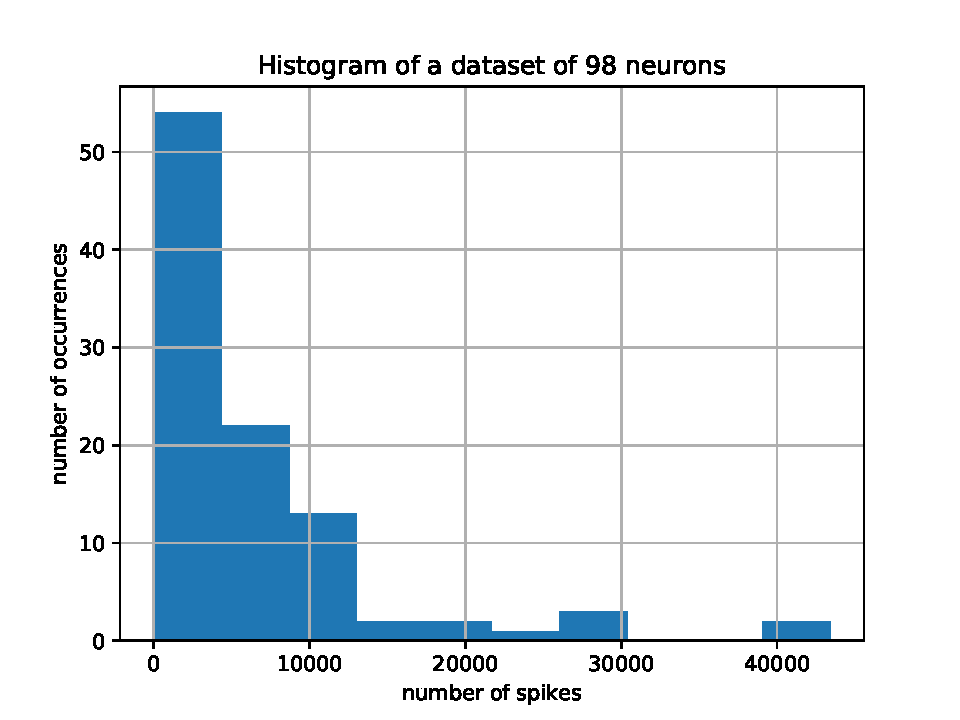
\includegraphics[width=0.8\textwidth]{histogram_number_spikes_dataset.pdf}
	\caption{Histogram of the number of spikes in a network of 98 neurons}
	\label{fig:histogram_spikes}
\end{figure}


\section{Differences between the real and simulated biological neural network}
\section{Input stimulus to the system}
\subsection{System with random spikes}
\subsection{System with randomly spiking clusters}
\section{Cascade generation}
\subsection{Method of maximum cascades}
\subsection{Method of maximum independence}
\subsection{Optimal cascade generation}
